\documentclass[11pt]{beamer} %

\usetheme{CambridgeUS}
\usecolortheme{dolphin}
\usepackage{times}
\usepackage{tikz}
\usepackage{amsmath}
\usepackage{verbatim}
\usepackage{algorithm,algorithmic}
%\usepackage{ctex}
\usepackage{filecontents,datatool}
\usepackage{lmodern}
\renewcommand*\familydefault{\sfdefault} %% Only if the base font of the document is to be sans serif
\usepackage[T1]{fontenc}

\renewcommand{\dtldisplaystarttab}{\toprule}

% likewise for \midrule and \bottomrule from booktabs 
\renewcommand{\dtldisplayafterhead}{\midrule}
\renewcommand{\dtldisplayendtab}{\\\bottomrule}

\newcommand*{\mat}[1]{\boldsymbol{\mathrm{#1}}}
\renewcommand*{\vec}[1]{\boldsymbol{#1}}

\usepackage{booktabs}
\usepackage{ulem}
\usepackage{subcaption}
\usepackage{listings}
\lstset{escapeinside=``, breaklines=true, frame=none, extendedchars=false, basicstyle=\ttfamily, showstringspaces=false}
\usefonttheme{professionalfonts}
\usetikzlibrary{arrows,shapes,positioning}
\newcounter{cont}
\makeatletter
%allowframebreaks numbering in the title
\setbeamertemplate{frametitle continuation}{%
    \setcounter{cont}{\beamer@endpageofframe}%
    \addtocounter{cont}{1}%
    \addtocounter{cont}{-\beamer@startpageofframe}%
    (\insertcontinuationcount/\arabic{cont})%
}
\makeatother
\linespread{1.2}
\author[Mengyun Chen, Yuge Zhang]{Mengyun Chen \quad 716030210013 \texorpdfstring{\\ Yuge Zhang \quad 716030210014}{}}
\date{June 14, 2018}

\begin{document}

\title[CS420 Project]{CS420 Machine Learning \\ Project: on MNIST dataset}

% For every picture that defines or uses external nodes, you'll have to
% apply the 'remember picture' style. To avoid some typing, we'll apply
% the style to all pictures.
\tikzstyle{every picture}+=[remember picture]

% By default all math in TikZ nodes are set in inline mode. Change this to
% displaystyle so that we don't get small fractions.
\everymath{\displaystyle}

\begin{frame}
\titlepage % Print the title page as the first slide
\end{frame}

\begin{frame}
\frametitle{Analysis}
\begin{itemize}
    \item Dataset technical specifications
        \begin{enumerate}
        \item Training sample size: 60000.
        \item Features: $45 \times 45$.
        \item Color: Grey. Integer range in $[0, 255]$.
        \item Labels: Integer in $[0,9]$.
        \item Test sample size: 10000.
        \end{enumerate}
        
    \item Difference from standard MNIST dataset
        \begin{enumerate}
        \item The image is randomly extended with black blocks.
        \item Some random noise has been added to the image.
        \end{enumerate}
\end{itemize}

\end{frame}


\begin{frame}
\frametitle{Preprocessing}
\begin{itemize}
    \item Centering: $45 \times 45 \rightarrow 32 \times 32$.
    \begin{figure}[htbp]
    \centering
    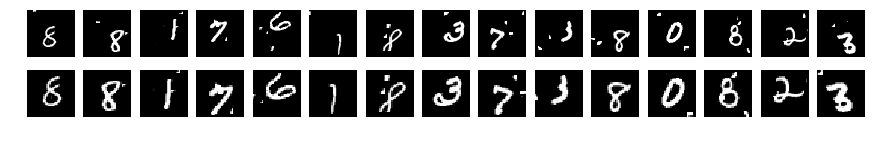
\includegraphics[width=1.0\linewidth]{img/centralize.png}
    \end{figure}
    
    \item Thresholding: $[0, 255] \rightarrow \{0, 1\}$.
    
    \item Helpful? Hopeless?
\end{itemize}

\end{frame}

\begin{frame}
\frametitle{Some approaches everyone might try...}
\begin{itemize}
    \item $k$-Nearest Neighbors?
    \item Support Vector Machine?
    \item Simple Neural Network provided by sklearn?
    \item PCA?
    \begin{itemize}
        \item Speedup?
        \item Improve accuracy?
    \end{itemize}
\end{itemize}
\end{frame}

\begin{frame}
\frametitle{Experiments -- MLP, kNN, SVM}
\begin{table}[htbp]
    \centering
    \begin{tabular}{cccc}
    \toprule
        Method & Preprocess & Accuracy & Time (second)  \\
    \midrule
        MLP & None & 0.6027 & 296.6  \\
        MLP + PCA & None & 0.8372 & 100.6  \\
        MLP + PCA & Centering & 0.9432 & 112.7  \\
    \midrule
        kNN & Thresholding & 0.7057 & 368.5  \\
        kNN & Centering & 0.9306 & 196.9  \\
        kNN & Thres + Cent & 0.9011 & 161.3 \\ 
    \midrule
        SVM + PCA & Thresholding & 0.882 & 353.3  \\
        SVM + PCA & Centering & \textbf{0.9678} & 144.1  \\
        SVM + PCA & Thres + Cent & 0.9641 & 147.4  \\
    \bottomrule
    \end{tabular}
\end{table}
\end{frame}


\begin{frame}[allowframebreaks]{CNN: Another approach everyone might try}

A reimplemented version with Tensorflow low-level API. No dropout.

\begin{figure}[htbp]
\centering
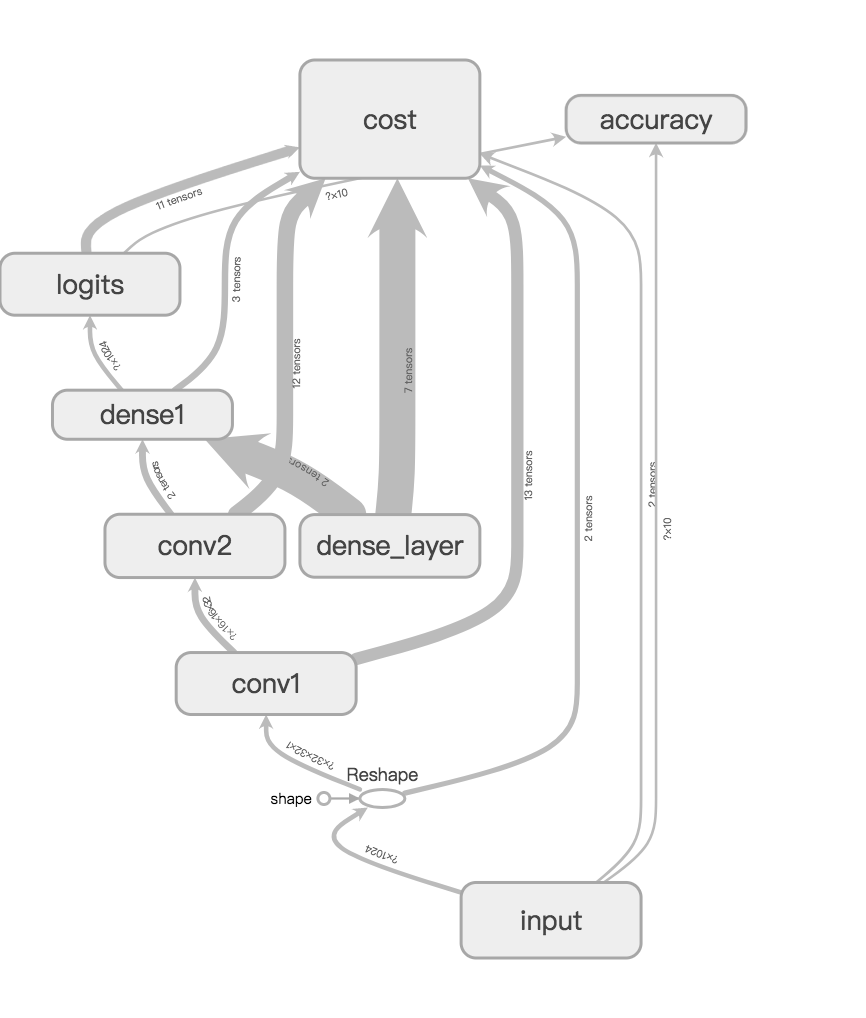
\includegraphics[width=0.4\textwidth]{img/cnn1.png}
\end{figure}    

\framebreak

\DTLloadrawdb{cnn2}{csv/cnn3.csv}

\begin{table}[htbp]
\centering
\DTLdisplaydb{cnn2}
\end{table}

\framebreak

Performance depends on training sample size?

\begin{figure}[htbp]
\centering
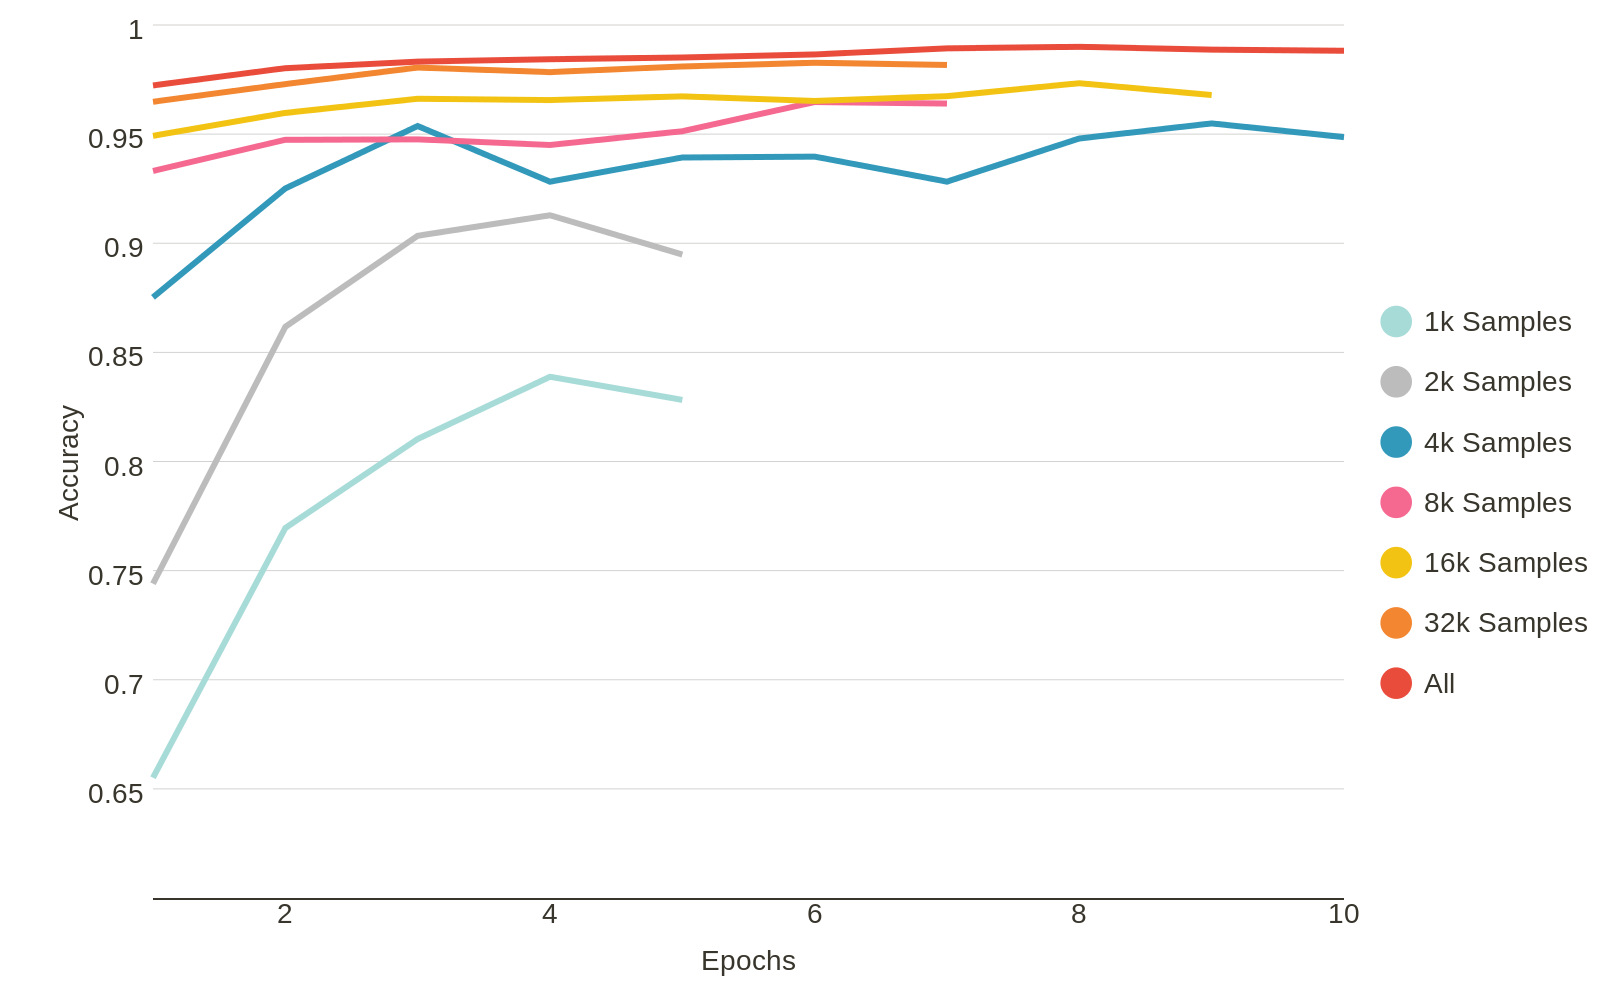
\includegraphics[width=0.8\textwidth]{img/cnn_sample_size.png}
\end{figure}
\end{frame}

\begin{frame}{Variational Autoencoder (VAE)}
\begin{enumerate}
    \item Unsupervised. So... bad idea?
    \item Replace PCA.
    \item Denoise.
    \item Fancy visualization.
\end{enumerate}
\end{frame}

\begin{frame}{VAE Network Architecture}
\begin{figure}[htbp]
\centering
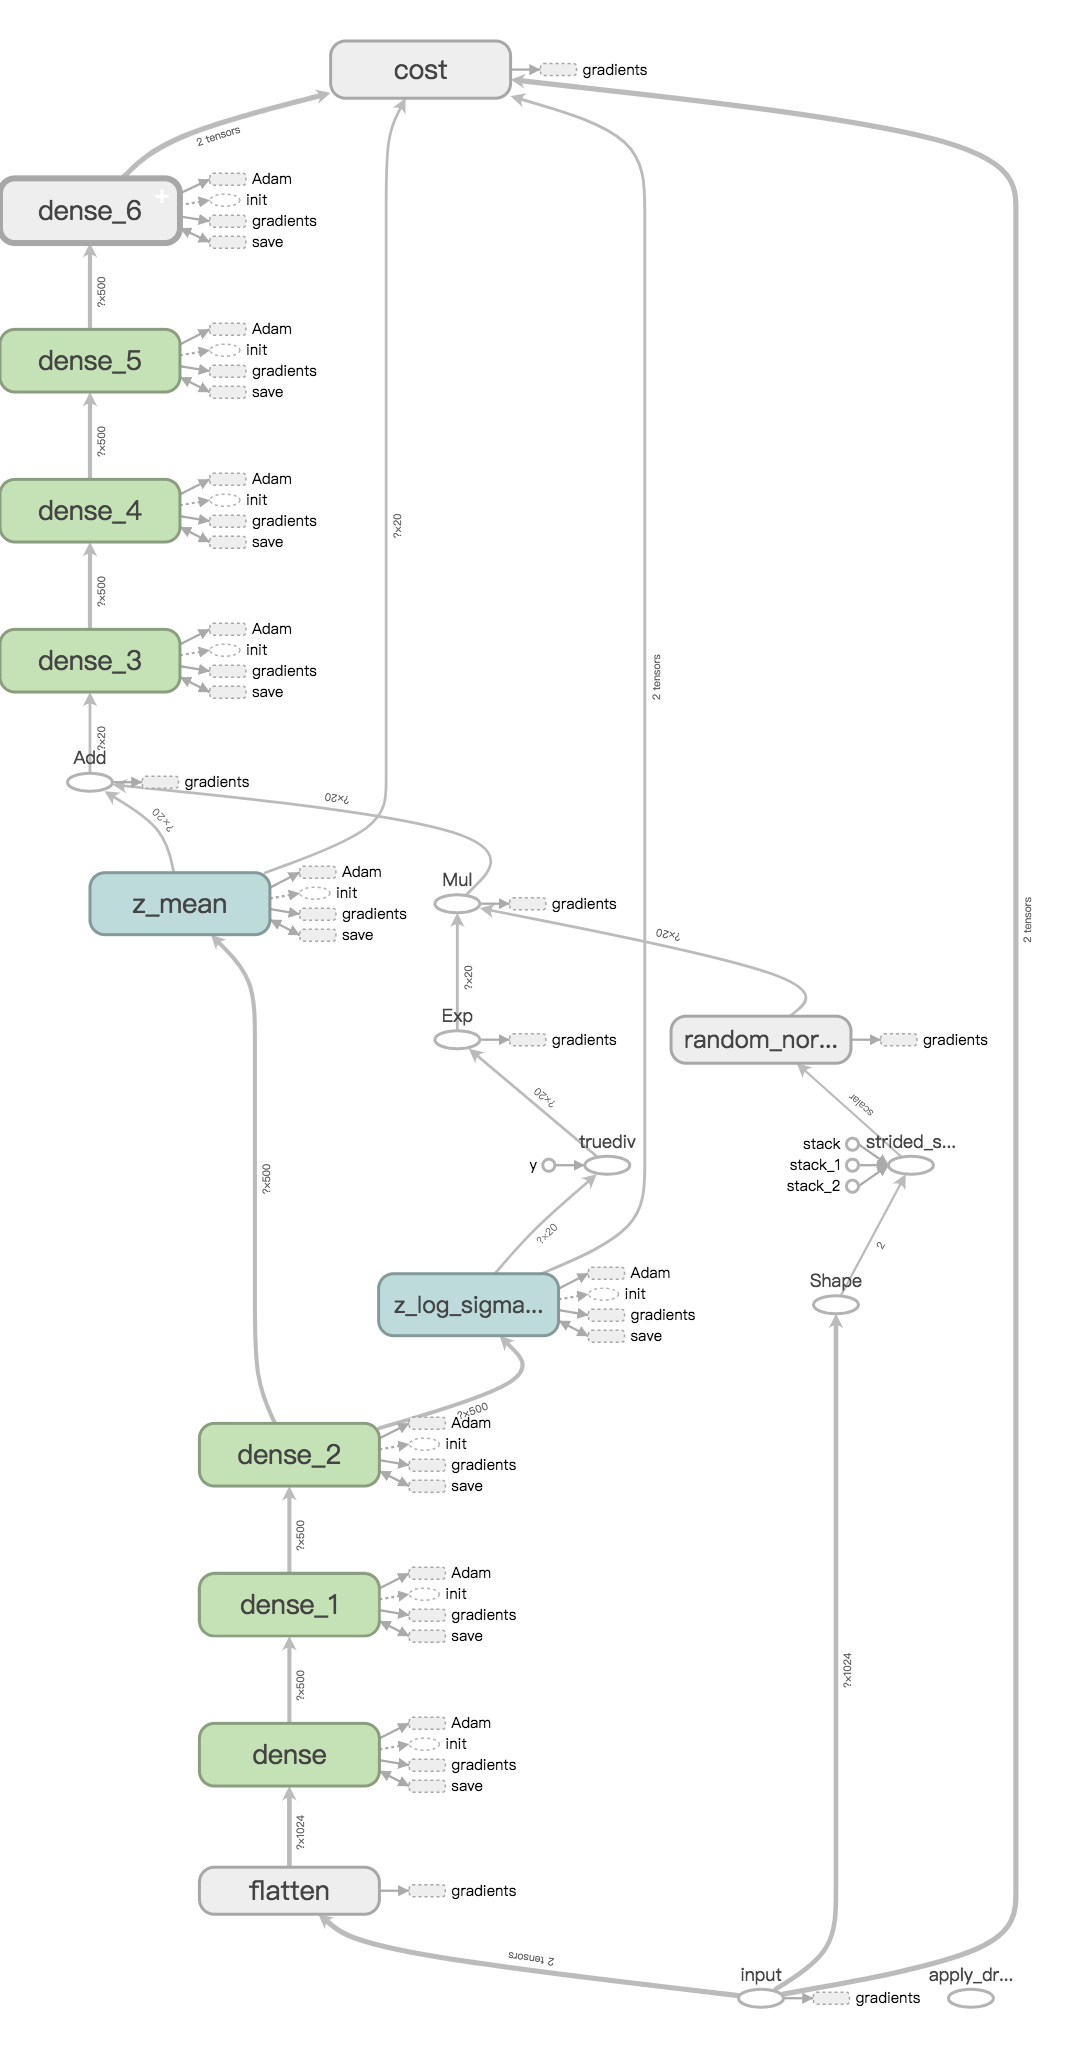
\includegraphics[width=0.5\textwidth,angle=-90,origin=c]{img/vae1.png}
\end{figure}
\end{frame}


\begin{frame}{VAE: Dimensionality reduction}
Dimension of latent space = 2.
\begin{figure}
    \centering
    \begin{subfigure}[h]{0.46\linewidth}
        \centering
        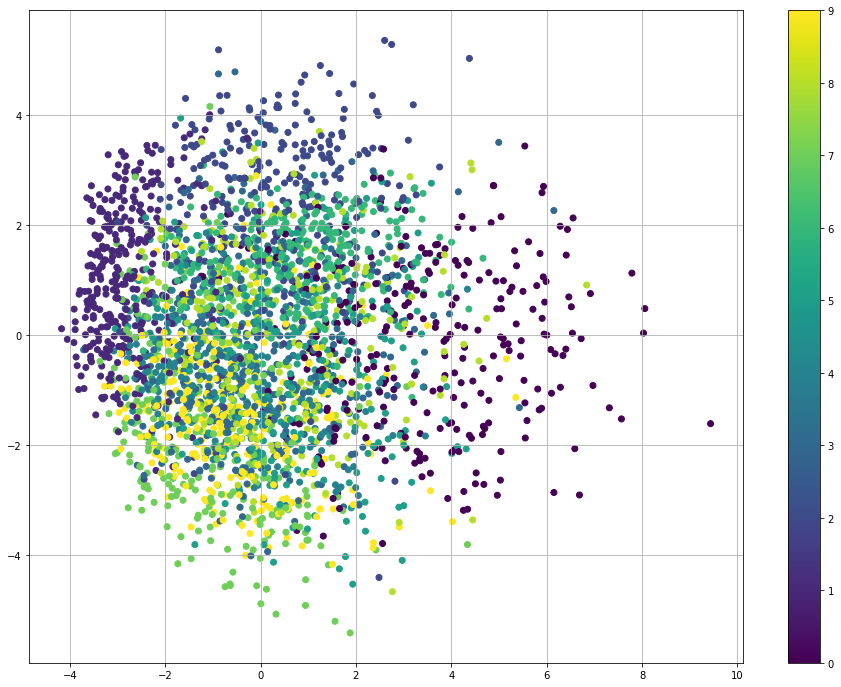
\includegraphics[width=0.75\textwidth]{img/dimreduce_pca.png}
        \caption{Result with PCA}
    \end{subfigure}
    \begin{subfigure}[h]{0.46\linewidth}
        \centering
        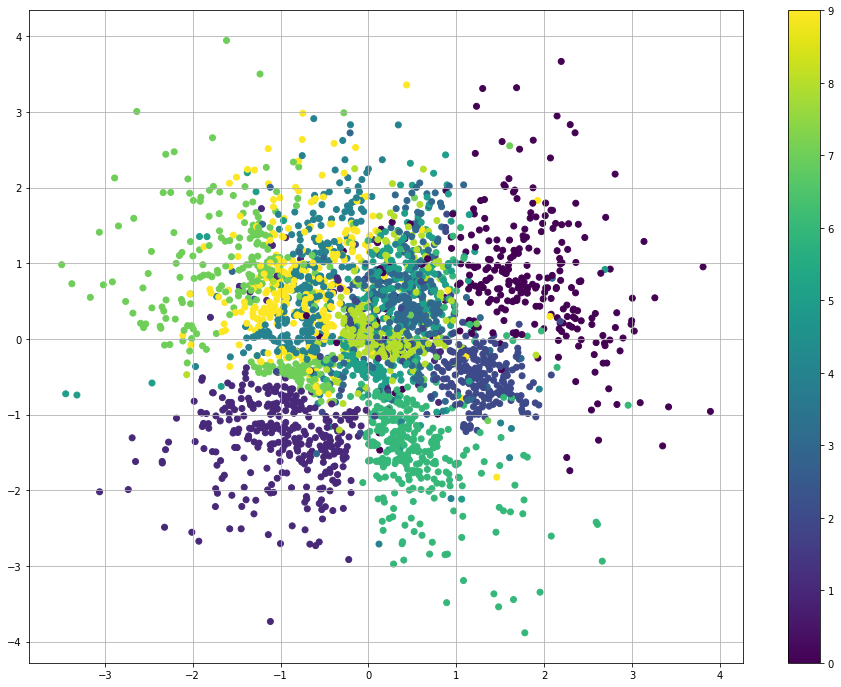
\includegraphics[width=0.75\textwidth]{img/dimreduce_vae.png}
        \caption{Result with VAE}
    \end{subfigure}
\end{figure}
\end{frame}


\begin{frame}{VAE: Reconstruction}
\begin{figure}[htbp]
\centering
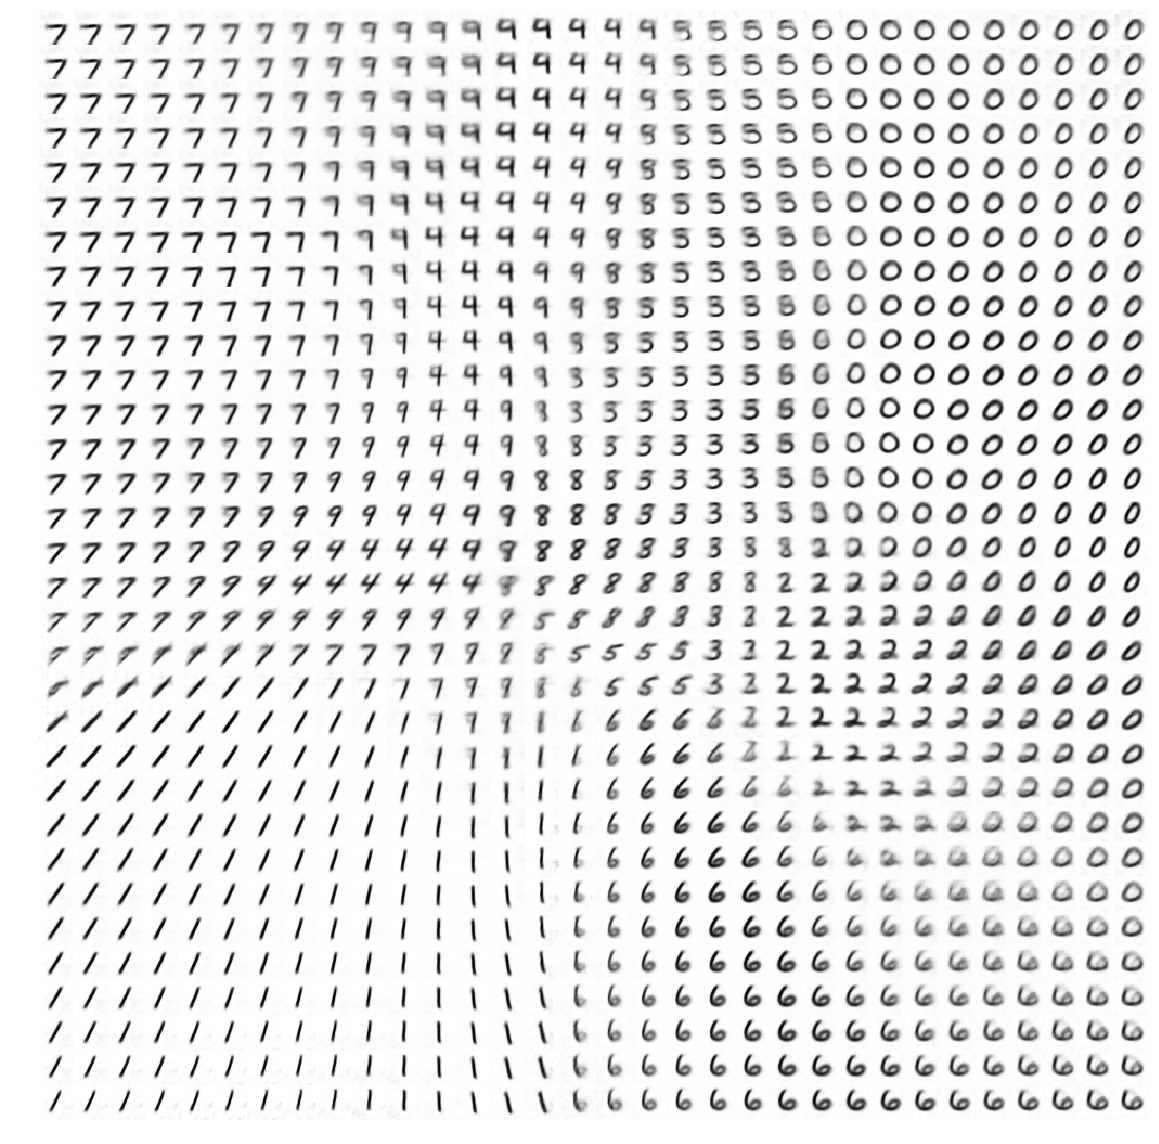
\includegraphics[width=0.6\textwidth]{img/reconstr_2d.png}
\end{figure}
\end{frame}


\begin{frame}{VAE: With CNN}
\begin{figure}[htbp]
\centering
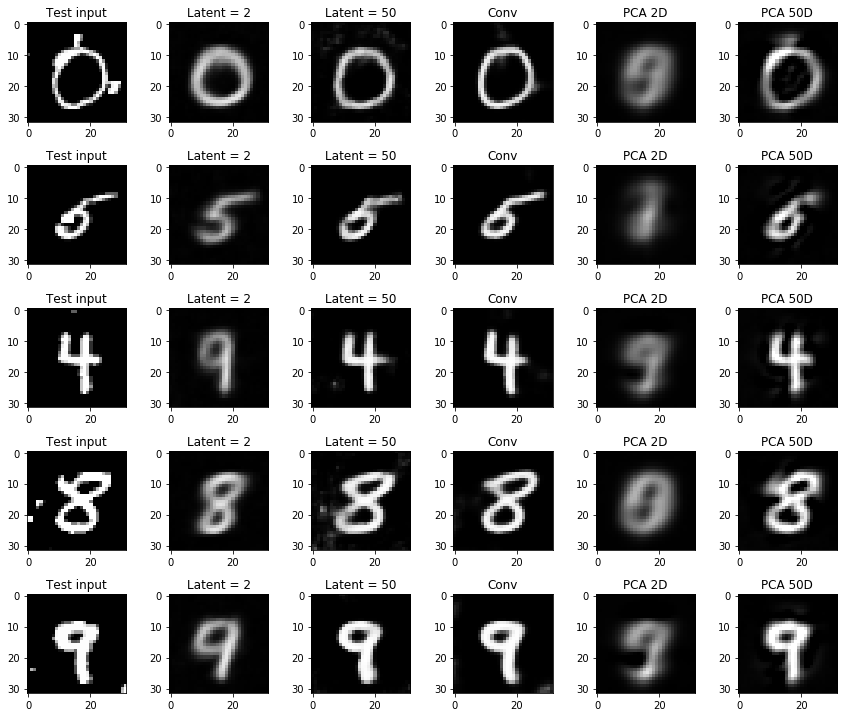
\includegraphics[width=0.55\textwidth]{img/reconstr_compare_pca_slides.png}
\caption{VAE 2D / VAE 50D / VAE CNN / PCA 2D / PCA 50D}
\end{figure}
\end{frame}

\begin{frame}{VAE: Helps classification}
\begin{itemize}
    \item Work as PCA.
    \item Use SVM in the following step.
\end{itemize}

\begin{table}[htbp]
    \centering
    \begin{tabular}{cccc}
    \toprule
        Method & Preprocess & Accuracy & Time  \\
    \midrule
        VAE + SVM (latent dim = 2) & Centering & 0.6944 & $\approx$ 7 mins \\
        VAE + SVM (latent dim = 50) & Centering & 0.9403 & $\approx$ 10 mins  \\
        VAE (Conv) + SVM & Centering & \textbf{0.9634} & $\approx$ 8 hours \\
    \bottomrule
    \end{tabular}
\end{table}

\end{frame}


\begin{frame}{Conditional Variational Auto Encoder}
Control the label and generate different styles of a number.
\begin{figure}
    \centering
    \begin{subfigure}[h]{0.45\linewidth}
        \centering
        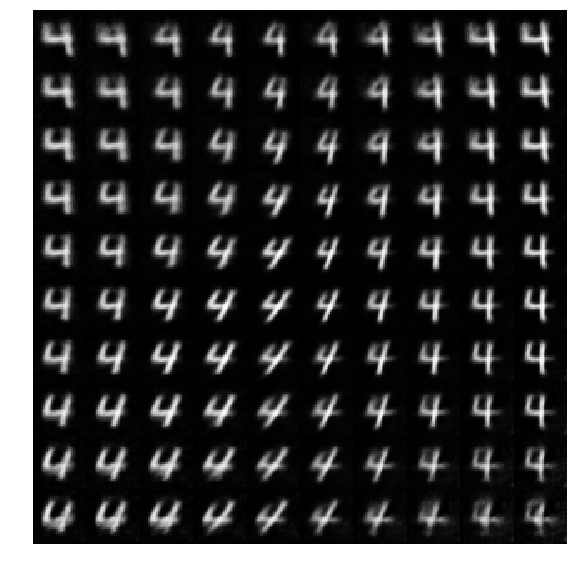
\includegraphics[width=1.0\textwidth]{img/cvae_4.png}
        \caption{Different styles of 4}
    \end{subfigure}
    \begin{subfigure}[h]{0.45\linewidth}
        \centering
        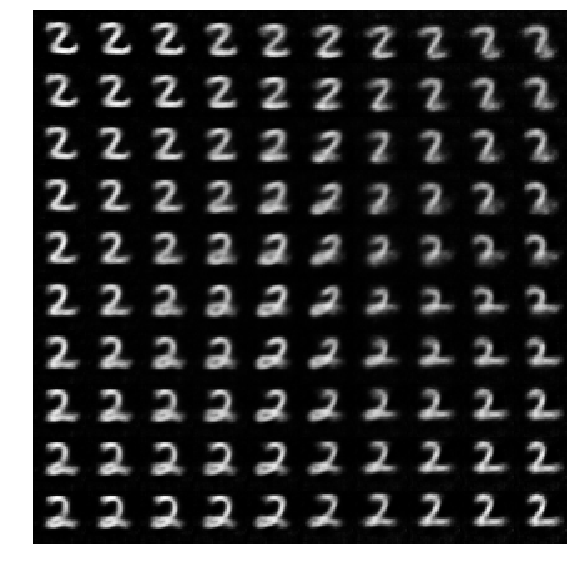
\includegraphics[width=1.0\textwidth]{img/cvae_2.png}
        \caption{Different styles of 2}
    \end{subfigure}
\end{figure}
\end{frame}

\begin{frame}[allowframebreaks]{CVAE: Classification}

\begin{algorithm}[H]
\caption{\textsc{Predict}($x$)}
\begin{algorithmic}
\REQUIRE{$\vec{x}$ is a $n$-dimension vector.}
\FORALL{$y$ in $[0,9]$ \AND $y$ is an integer}
    \STATE regenerate $\vec{x'}$ with $(\vec{x}, y)$.
    \STATE \textsc{BestLoss} $\leftarrow \infty$
    \IF {\textsc{ReconstrLoss}$(\vec{x}, \vec{x'})$ $<$ \textsc{BestLoss}}
        \STATE \textsc{BestLoss} $\leftarrow$ \textsc{ReconstrLoss}$(\vec{x}, \vec{x'})$
        \STATE \textsc{Label} $\leftarrow y$
    \ENDIF
\ENDFOR
\RETURN \textsc{Label}
\end{algorithmic}
\end{algorithm}

\framebreak

\begin{itemize}
    \item $\textsc{ReconstrLoss} = \vec{x} \log (\vec{x'}) + (1 - \vec{x}) \log (1 - \vec{x'})$.
    \item Hit accuracy \textbf{0.9423} with 3 layers, 500 hidden units each, 20-dimension latent space and 15-minute training.
    \item Disappointing?
\end{itemize}

\framebreak

\begin{figure}[htbp]
\centering
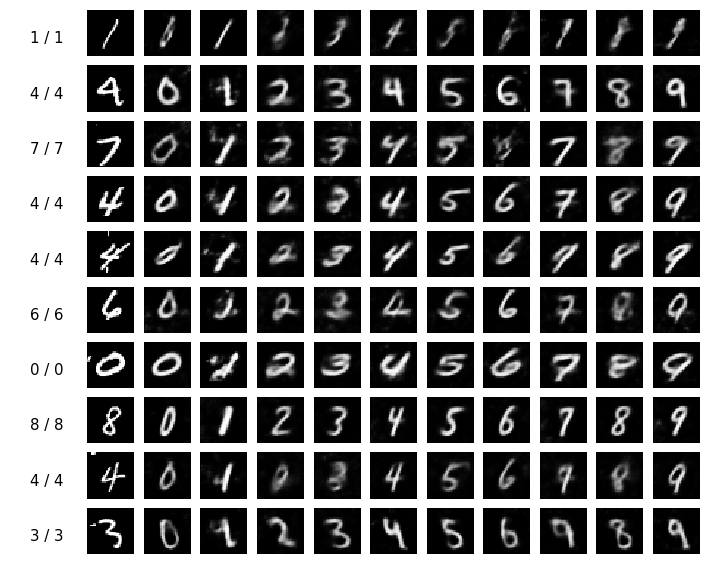
\includegraphics[width=0.6\textwidth]{img/cvae_reconstr.png}
\caption{CVAE reconstruction with label from 0 to 9}
\label{fig:cvae_reconstr}
\end{figure}

\framebreak

\textit{}

\begin{figure}[htbp]
\centering
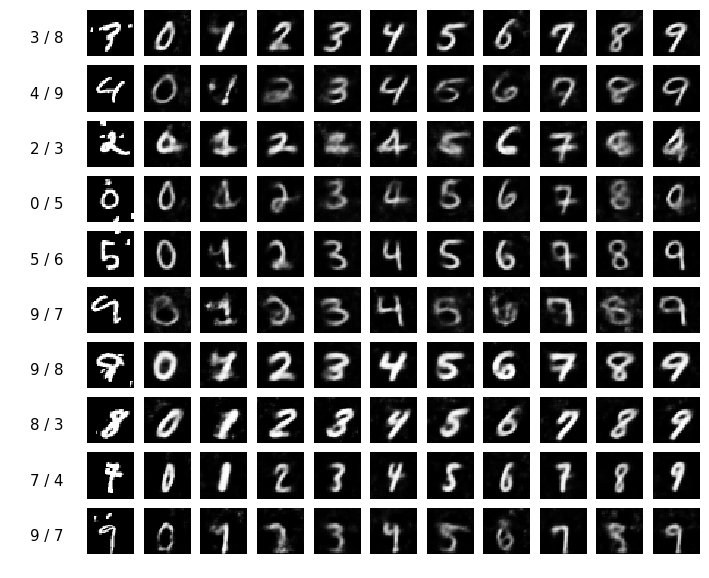
\includegraphics[width=0.58\textwidth]{img/cvae_reconstr_error.png}

\textit{CVAE: It doesn't look like anything to me...}
\end{figure}

\end{frame}

\begin{frame}{Something else?}

\begin{itemize}
    \item Lack of fundings, we didn't use any GPU. All the tests on done on a server with Intel Xeon CPU E5-2650 v4 @ 2.20GHz with 24 cores and 32 GB RAM.
    \item The math behind VAE is responsible for a lot of headaches. Luckily, programming is easier than math...
    \item The project was designed to be simple, straight-forward, clichéd. It turned out to be way much more time-consuming and fascinating than expected.
\end{itemize}
    
\end{frame}



\end{document}
              